\begin{figure*}[!ht]
  \centering
  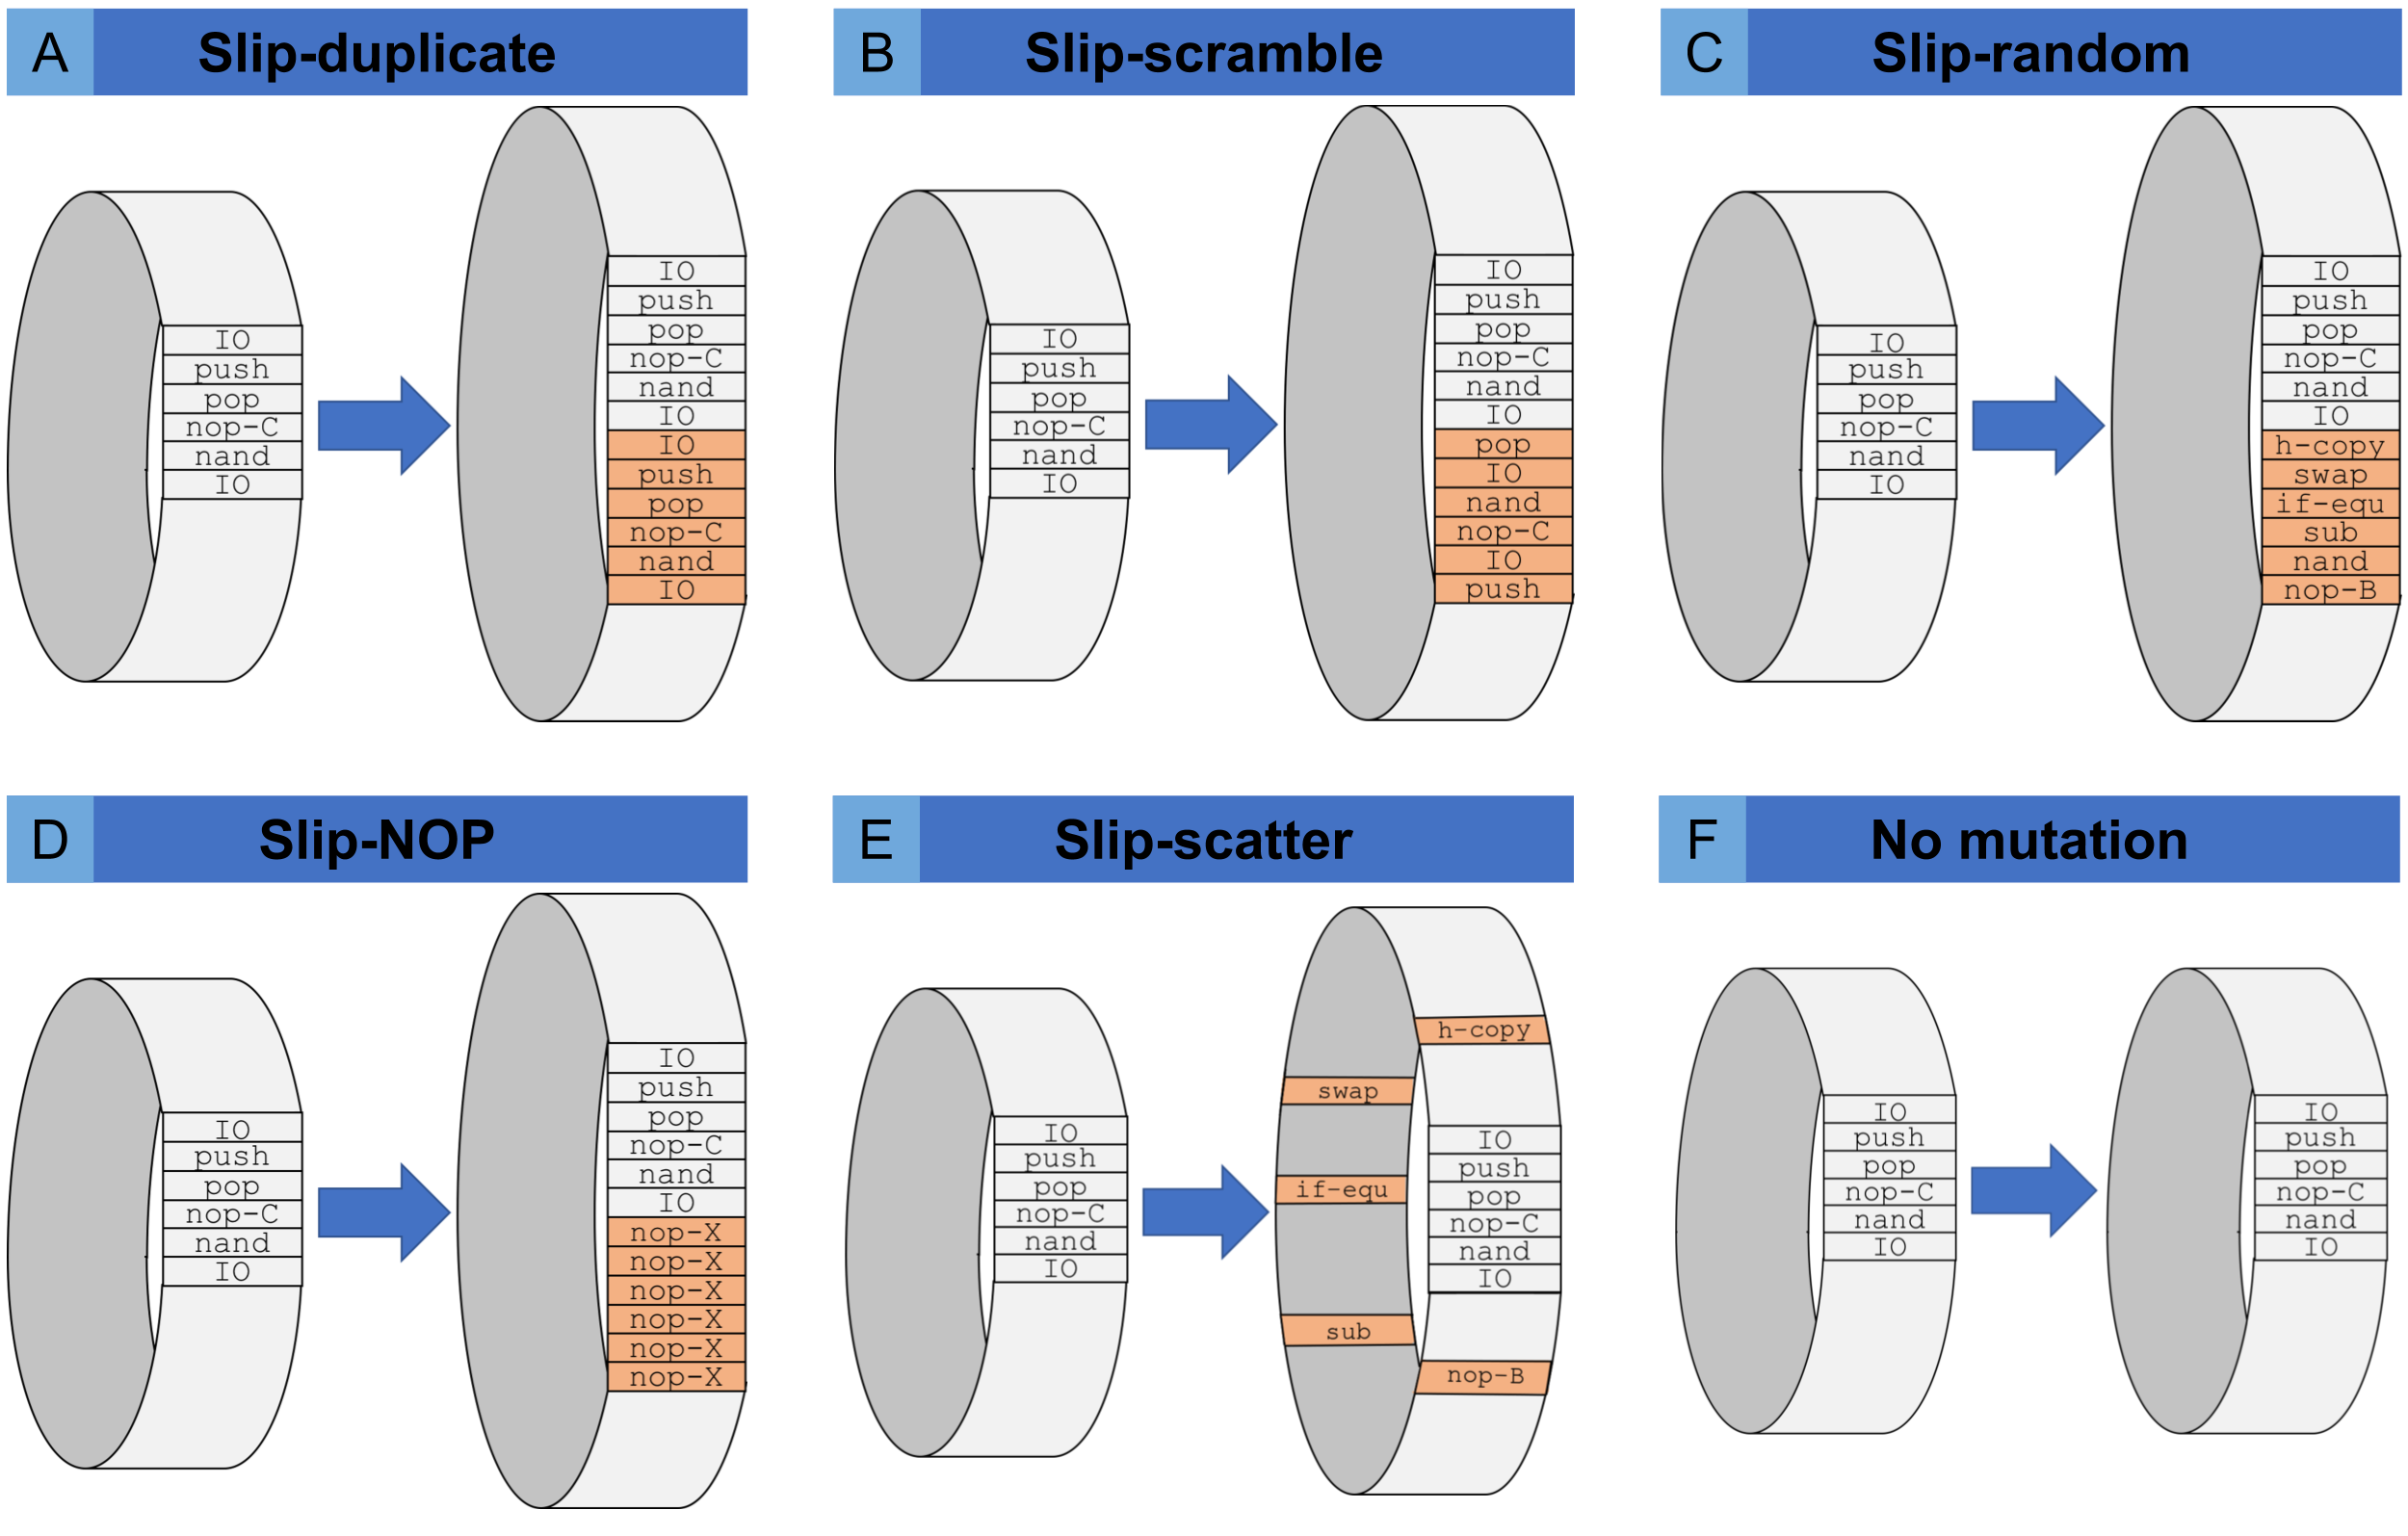
\includegraphics[width=\textwidth]{imgs/slip_mutation_variants.png}
   % 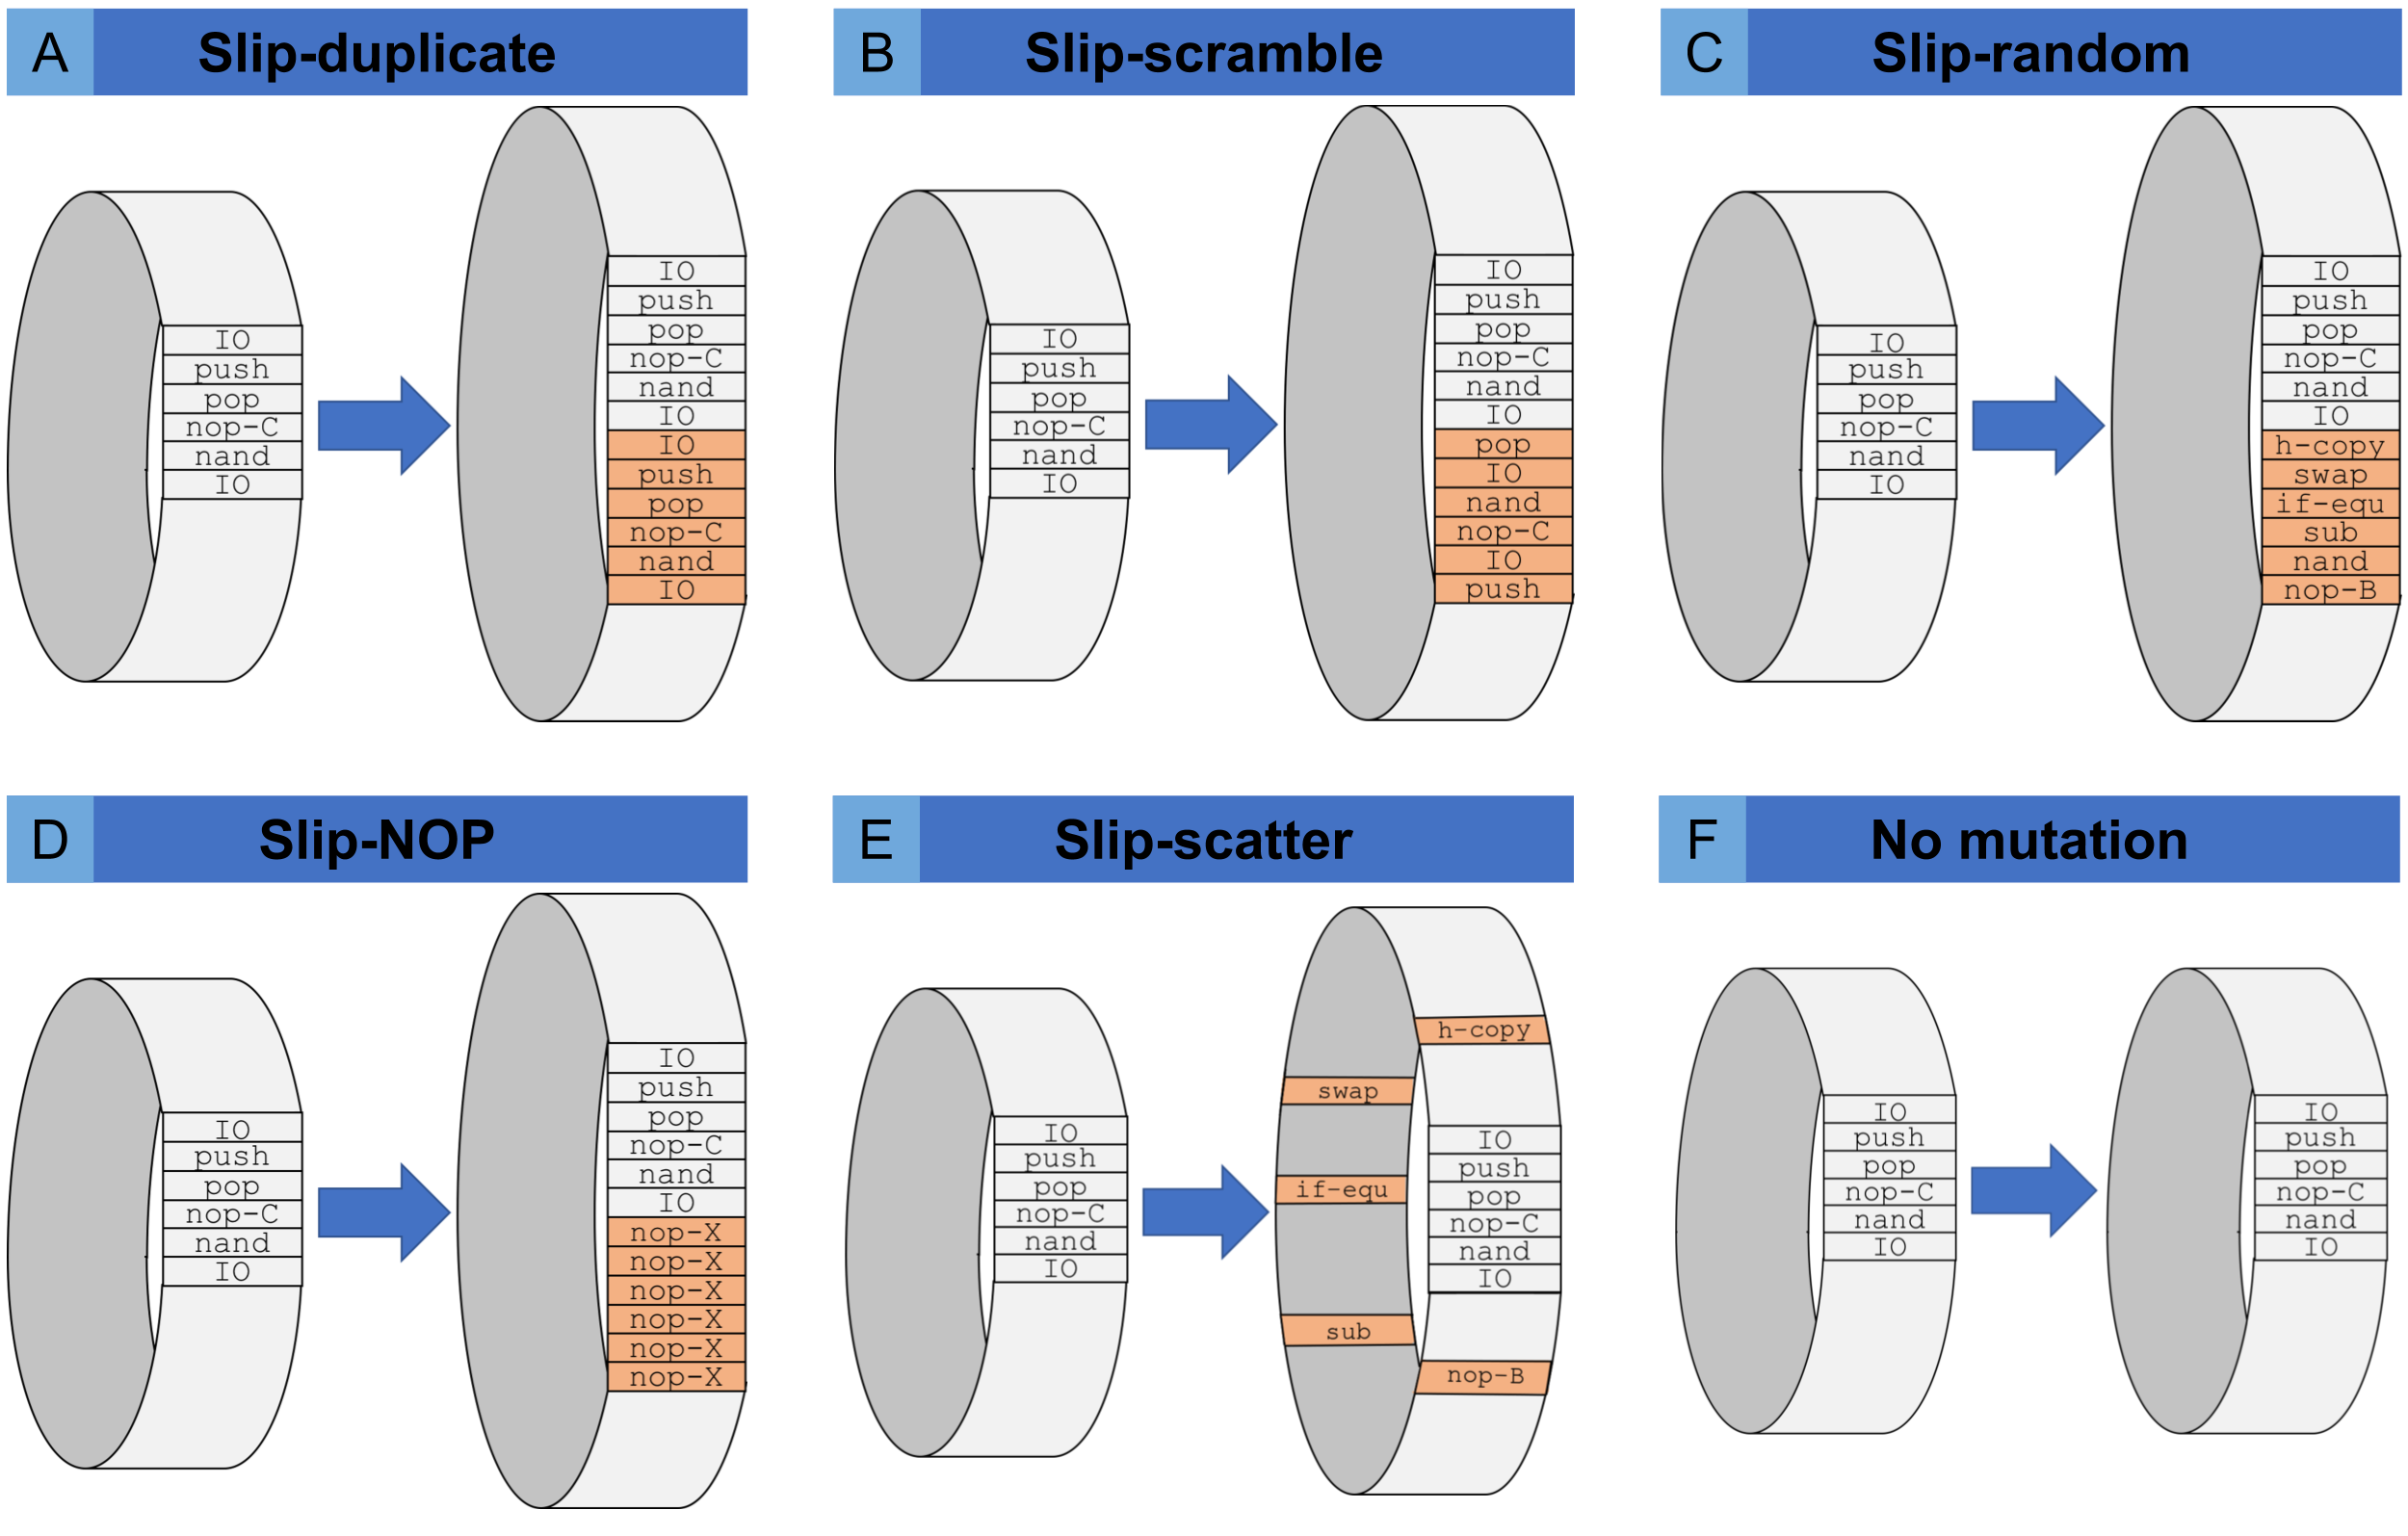
\includegraphics[height=0.4\textheight]{imgs/slip_mutation_variants.png}
    \caption{
    \textbf{Surveyed slip mutation operators.}
    A) Slip-duplicate: an exact duplication is inserted adjacent to the target segment.
    B) Slip-scramble: shuffled duplication is inserted directly after the target segment.
    C) Slip-random: random instructions are inserted directly after the target segment.
    D) Slip-NOP: neutral nop-X instructions are inserted directly after the target segment.
    E) Slip-scatter: randomly-drawn instructions are inserted at random throughout the genome.
    F) slip mutation disabled. }
    \label{fig:slip_mut_variants}
\end{figure*}
